\chapter{Конструкторский раздел}

В данном разделе будут представлены этапы проектирования базы данных, выделены конкретные действия ролевой модели, спроектирован триггер и интерфейс взаимодействия.

\section{Формализация сущностей системы}

На основе выделенных ранее сущностей спроектированы следующие таблицы базы данных.
\begin{enumerate}
	\item Таблица User -- содержит информацию о пользователях системы. Включает следующие поля:
	\begin{itemize}
		\item tgName -- имя пользователя в telegram, символьный тип, является идентификатором;
		\item geoLat, geoLong -- местоположение пользователя, вещественный тип;
		\item customerRole, executorRole, administratorRole -- наличие у пользователя описываемой роли, логический тип;
		\item adminVerified -- статус подтверждения роли администратора у пользователя, логический тип.
	\end{itemize}
	\item Таблица Connection -- содержит информацию о подключениях пользователей под определенной ролью. Включает следующие поля:
	\begin{itemize}
		\item userTgName -- идентификатор пользователя, целочисленный тип;
		\item currentRole -- текущая роль, символьный тип.
	\end{itemize}
	Совокупность этих полей является идентификатором подключения.
	\item Таблица Request -- содержит информацию о заявках системы. Включает следующие поля:
	\begin{itemize}
		\item id -- идентификатор заявки, целочисленный тип;
		\item title -- название заявки, символьный тип; 
		\item periodOfRelevance -- срок релевантности заявки, временная метка;
		\item explanation -- пояснение к заявке, символьный тип;
		\item profNecessity -- необходимый проф. навык, идентификатор навыка, целочисленный тип;
		\item equipment -- необходимое оборудование, идентификатор оборудования, целочисленный тип; 
		\item owner, executor -- оформитель и исполнитель, идентификатор пользователя, символьный тип;
		\item status -- статус заявки, символьный тип.
	\end{itemize}
	\item Таблица Equipment -- содержит информацию об используемом оборудовании. Включает следующие поля:
	\begin{itemize}
		\item id -- идентификатор оборудования, целочисленный тип;
		\item name -- название оборудования, символьный тип.
	\end{itemize}
	\item Таблица Skill -- содержит информацию о навыках в системе. Включает следующие поля:
	\begin{itemize}
		\item id -- идентификатор навыка, целочисленный тип;
		\item name -- название навыка, символьный тип.
	\end{itemize}
	\item Таблица ExecutorSkill -- реализует связь <<многие ко многим>> исполнителей и навыков. Включает следующие поля:
	\begin{itemize}
		\item executorId -- идентификатор пользователя (исполнителя), символьный тип;
		\item skillId -- идентификатор навыка, целочисленный тип;
		\item status -- статус подтвержденния навыка, символьный тип.
	\end{itemize}
	Совокупность executorId и skillId является идентификатором данной таблицы.
	%\item Таблица EquipmentSkill -- реализует связь <<многие ко многим>> оборудования и навыков. Включает следующие поля:
	%\begin{itemize}
	%	\item equipmentId -- идентификатор оборудования, целочисленный тип;
	%	\item skillId -- идентификатор навыка, целочисленный тип.
	%\end{itemize}
	%Совокупность этих полей является идентификатором данной таблицы.
	\item Таблица Ban -- содержит части слов, по которым можно определить ненормативную лексику. Состоит из единственного поля word -- символьный тип, является идентификатором.
\end{enumerate}
\newpage
Соответствующая диаграмма по описанным выше данным представлена на рисунке \ref{er}.

\begin{figure}[H]
	\begin{center}
		\includegraphics[scale=0.68]{assets/er.png}
	\end{center}
	\caption{ER-диаграмма системы}
	\label{er}
\end{figure}

\section{Ролевая модель}

На уровне базы данных выделена следующая ролевая модель.
\begin{enumerate}
	\item Customer -- оформитель заявки. Обладает правами:
	\begin{itemize}
		\item INSERT/UPDATE над таблицами User, Connection;
		\item все права над таблицей Request;
		\item INSERT над таблицами Skill, Equipment.
	\end{itemize}
	\item Executor -- исполнитель заявки. Обладает правами:
	\begin{itemize}
		\item INSERT/UPDATE над таблицами User, Connection;
		\item SELECT/UPDATE над таблицей Request;
		\item INSERT над таблицами Skill, ExecutorSkill.
	\end{itemize}
	\item Administrator -- администратор. Обладает правами:
	\begin{itemize}
		\item все права над таблицами User, Connection;
		\item все права над таблицей ExecutorSkill;
		\item все права над таблицей Ban.
	\end{itemize}
\end{enumerate}
Использование ролевой модели на уровне базы данных гарантирует безопасность доступа к объектам.

Сценарий создания базы данных и выделение ролей представлены в приложение А.

\section{Триггер}

В системе предусмотрен механизм предотвращения использования ненормативной лексики. Он реализован вспомогательной таблицей Ban, хранящей части слов для распознавания,  а также триггером AFTER на действие INSERT в таблицу Request. Данный триггер проверяет наличие вхождений в заголовок (поле title) и пояснение (поле explanation) частей <<запрещенных>> слов.

На рисунке \ref{trigger} представлена схема алгоритма работы выполняемой триггером функции checkBanWords().

\begin{figure}[H]
	\begin{center}
		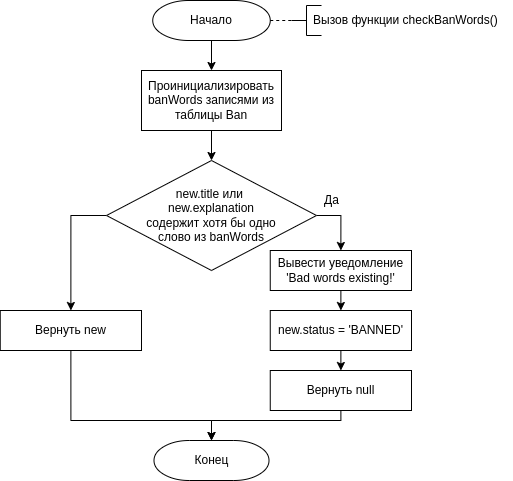
\includegraphics[scale=0.6]{assets/trigger.png}
	\end{center}
	\caption{Триггер AFTER на создание новой заявки}
	\label{trigger}
\end{figure}

\section{Проектирование приложения}

Приложение, обеспечивающее взаимодействие с базой данных, представляет собой telegram-бота. Использование имени пользователя в telegram в качестве первичного ключа является целесообразным, так как гарантируется уникальность данного параметра на уровне мессенджера. Разработка будет осуществляется в соответствии с принципами <<чистой архитектуры>> \cite{clear_code}. Использование такого подхода позволило выделить несколько компонентов: доступ к данным, бизнес-логика, транспортный уровень и  UI, реализуемый на основе telegramAPI \cite{telegram_api}. 
%Приложение также снабжено системой логирования.

\section{Вывод из раздела}

В данном разделе были описаны этапы проектирования базы данных и приложения.